\subsection{Projection Review}
\label{sec.projection_review}

%This section reviews the viewing transform used by most popular graphics frameworks such as OpenGL. 

%Yet there is no standard way to specify the view, and there are a wide range of different viewing implementations currently in use.

%Closely tied in to viewing parameters is 3D interaction, and there are likewise a large number of different 3D interaction implementations often providing the same basic functionality. Users are forced to learn and use different pan, zoom, and spin techniques for each 3D program they use. As every 3D program has to reinvent this functionality,  OpenGL standard has emerged to supply the lack of standardization, the need of higher development and support efforts; as well as stifling the proliferation of user interface features like stereo. A standard viewing software toolkit, along with a standard motion toolkit, would benefit end users by delivering consistent and comprehensive 3D interaction across applications, and would benefit developers by reducing development time, software support, and customer support. All of the various interaction techniques can be provided to satisfy the varying requirements of the different types of 3D programs and the different levels of end user expertise.

Generation of 3D computer graphics is essentially a straightforward mapping of graphical items in a 3D view volume to a 2D image. Most viewing software use different transforms combined to deliver consistent and comprehensive 3D interactions: the model transform represents the individual transformations that represents the individual transformations of each object in the 3D scene; which is the mapping $M_{model}: S_{model} \Rightarrow S_{scene}$ in the model and scene spatial domains in $\Re^3$; the view transform represents the individual transformations of every object in the 3D scene, representing the scene positioning for the viewer; which is the mapping $M_{view}: S_{scene} \Rightarrow S_{view}$ in the model and scene domains in $\Re^3$; and the projection transform is the mapping $M_{projection}:S_{view} \Rightarrow S_{projection}$ that represents the transform of a view of scene in $\Re^3$. The latter domain in then mapped to screen coordinates using a viewport transform $M_{viewport}:S_{projection} \Rightarrow S_{screen}$ into the domain of the screen in $\Re^2$.

%The combination of the first and second transforms, view and model, is a single transform that translates and rotates the scene accordingly the viewer position, looking direction and view roll. This is an affine transform and the inverse  transform exists. Both transforms can be easily computed as a matrix in homogeneous coordinates. The latter transform projects the 3D scene into the output image. In most cases, the output image is a rectangular shape and the 3D view volume, called frustum, which is either a rectangular prism or a truncated pyramid for parallel and perspective views, respectively.

In the OpenGL framework, the model and view transforms are combined in the \verb|GL_MODELVIEW| matrix. The 3D scene rendered by OpenGL must then be projected onto the computer screen as a 2D image using the \verb|GL_PROJECTION| matrix. First, it transforms all vertex data from the eye coordinates to the clip coordinates. Then, these clip coordinates are also transformed to the Normalized Device Coordinates (NDC) dividing by the $w$ component of the clip coordinates.

\begin{figure}[h!]
\centering
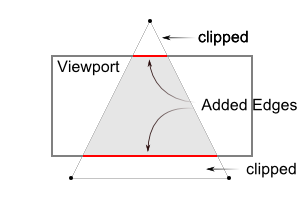
\includegraphics[width=0.9\linewidth,keepaspectratio=true]{figs/gl_frustumclip.png}
\caption{A triangle clipped by frustum}
\label{fig.clipping}
\end{figure}

Bear in mind that both clipping (frustum culling) and NDC transformations are integrated into \verb|GL_PROJECTION| matrix, as illustrated in Figure~\ref{fig.ndc}. The following sections describe how to build the projection matrix from 6 parameters; left, right, bottom, top, near and far boundary values.

Note that the frustum culling (clipping) is performed in the clip coordinates, just before dividing by $w_c$. The clip coordinates, $x_c$, $y_c$ and $z_c$ are tested by comparing with $w_c$. If any clip coordinate is less than $-w_c$, or greater than $w_c$, then the vertex will be discarded. Then, OpenGL will reconstruct the edges of the polygon where clipping occurs.

In perspective projection, a 3D point in a truncated pyramid frustum (eye coordinates) is mapped to NDC; which is a cube with the range of $x$-coordinate from $[l, r]$ to $[-1, 1]$, the y-coordinate from $[b, t]$ to $[-1, 1]$ and the $z$-coordinate from $[n, f]$ to $[-1, 1]$.

Note that the eye coordinates are defined in the right-handed coordinate system, but NDC uses the left-handed coordinate system. That is, the camera at the origin is looking along $-Z$ axis in eye space, but it is looking along $+Z$ axis in NDC.

Since glFrustum() accepts only positive values of near and far distances, they are negated during the construction of \verb|GL_PROJECTION| matrix.

\begin{figure}[h!]
\centering
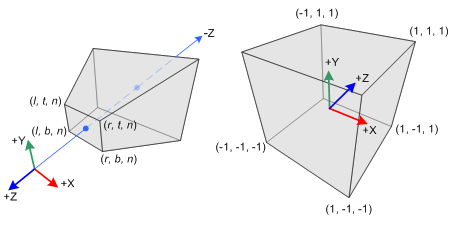
\includegraphics[width=0.9\linewidth,keepaspectratio=true]{figs/gl_projectionmatrix01.png}
\caption{Perspective Frustum and Normalized Device Coordinates (NDC)}
\label{fig.ndc}
\end{figure}

 The complete projection matrix is: 
\begin{equation}
\begin{aligned}
\begin{pmatrix} x_{c}\\y_{c}\\z_{c}\\w_{c} \end{pmatrix} &= 
\begin{pmatrix} 
\frac{2n}{r-l} & 0 & \frac{r+l}{r-l} & 0 \\
0 & \frac{2n}{t-b} & \frac{t+b}{t-b} & 0 \\
\cdot & \cdot & -\frac{f+n}{f-n} & -\frac{2fn}{f-n} \\
0 & 0 & -1 & 0 \\
\end{pmatrix} \\
\end{aligned}
\label{eq.projection_matrix}
\end{equation}


